% Figure for scale_lanes_deck: Offline sweep (harness_scaling_demo.py): throughput vs replicas.
% Build: xelatex lanes_fig07_sweep.tex  (-> .pdf, included by ../scale_lanes_deck.md)
\documentclass[tikz,border=4pt]{standalone}
\usepackage{fontspec}
\setmainfont{DejaVu Sans}
\setmonofont{DejaVu Sans Mono}
\usetikzlibrary{positioning,arrows.meta,fit,backgrounds,calc,decorations.pathreplacing}
\definecolor{slime}{RGB}{230,230,230}
\definecolor{host}{RGB}{214,216,240}
\definecolor{gpu}{RGB}{255,236,204}
\definecolor{vm}{RGB}{214,238,220}
\definecolor{ac}{RGB}{255,246,230}
\definecolor{bad}{RGB}{245,205,205}
\definecolor{ink}{RGB}{40,40,90}
\begin{document}
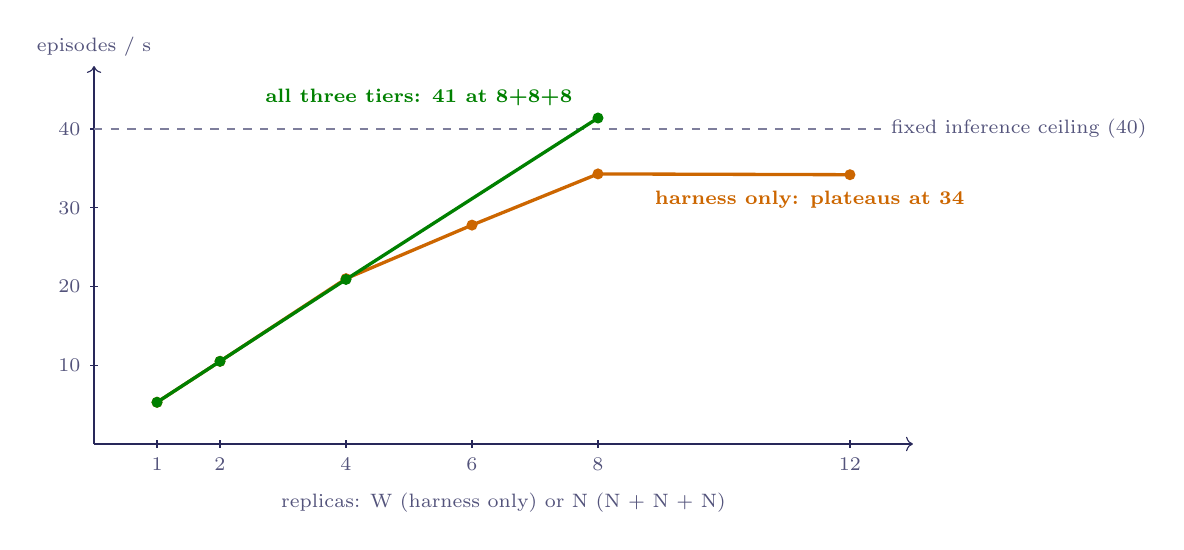
\begin{tikzpicture}[
  font=\footnotesize,
  box/.style={draw=ink, rounded corners=3pt, fill=#1, align=center, inner sep=4pt, minimum height=0.9cm, minimum width=2.8cm},
  line/.style={thick, draw=ink, -{Stealth[length=2mm]}},
  dline/.style={thick, draw=ink, {Stealth[length=2mm]}-{Stealth[length=2mm]}},
  head/.style={font=\small\bfseries, text=ink, align=center},
  lab/.style={font=\scriptsize, text=ink, fill=white, inner sep=1.5pt, align=center},
  note/.style={font=\scriptsize, text=ink!80, align=center},
  region/.style={draw=ink!60, dashed, rounded corners=6pt, inner sep=8pt},
]

% axes: x = N (1..12) at 0.8 cm per unit; y = ep/s at 0.1 cm per unit
\draw[->, ink] (0,0) -- (10.4,0);
\node[note] at (5.2,-0.75) {replicas: W (harness only) or N (N + N + N)};
\draw[->, ink] (0,0) -- (0,4.8) node[above, note] {episodes / s};
\foreach \x in {1,2,4,6,8,12} \draw[ink] (\x*0.8,0.05) -- (\x*0.8,-0.05) node[below, note] {\x};
\foreach \y in {10,20,30,40} \draw[ink] (0.05,\y*0.1) -- (-0.05,\y*0.1) node[left, note] {\y};
\draw[dashed, ink!60] (0,4.0) -- (10,4.0) node[right, note] {fixed inference ceiling (40)};
\draw[very thick, color=orange!80!black] plot coordinates {(0.8,0.53) (1.6,1.05) (3.2,2.10) (4.8,2.78) (6.4,3.43) (9.6,3.42)};
\foreach \p in {(0.8,0.53),(1.6,1.05),(3.2,2.10),(4.8,2.78),(6.4,3.43),(9.6,3.42)} \fill[orange!80!black] \p circle (2pt);
\draw[very thick, color=green!50!black] plot coordinates {(0.8,0.53) (1.6,1.05) (3.2,2.09) (6.4,4.14)};
\foreach \p in {(0.8,0.53),(1.6,1.05),(3.2,2.09),(6.4,4.14)} \fill[green!50!black] \p circle (2pt);
\node[font=\scriptsize\bfseries, text=orange!80!black, anchor=west] at (7.0,3.1) {harness only: plateaus at 34};
\node[font=\scriptsize\bfseries, text=green!50!black, anchor=east] at (6.2,4.4) {all three tiers: 41 at 8+8+8};
\end{tikzpicture}
\end{document}
